%This line is just a comment.  Ignore it!
%

\documentclass [12pt] {article}
\usepackage{graphicx}
\title{Showing the 2004 IUCF REU Students the Wonders of \LaTeX\ }
\date{\today}

\author{David P. Murdock}


\begin{document}
\maketitle

\begin{abstract}
In this article, I attempt to show the 2004 IU REU students the power of
computer typesetting.  I try to distinguish typesetting from word processing. I
ridicule those who use word processing for scientific documents.  I make rude
remarks; I insult their pets and relatives.  I make sure that they will {\it
never} use a regular word processor again. {\it Bwaaah--hah hahhh!}
\end{abstract}

\section {Introduction}

\subsection {Why Do We Use \LaTeX\ ?}

\LaTeX\ is a {\it typesetter}, not a word processor.  Word
processors are for girly--men.  Typesetters are for physicists with
pumpitude.

To make a new paragraph in \LaTeX\ , skip a line.

You have a choice of fonts in \LaTeX\ . You can print in {\it italics},
{\bf boldface}, {\sl slanted}, {\tt typewriter} and {\sf sans--serif}.


\subsection{\LaTeX\ Does Math!}

It sure does!  You can put mathematics inside of paragraphs:
 \( c=\sqrt{a^2+b^2} \), or you can {\it display} equations:
\[ \int_0^1 x^2 dx=  \frac {1} {3}   \qquad \qquad
\int \cos (x) dx= \sin(x) \]

It will automatically number equations too.
\begin{equation}
-{\hbar^2\over 2M}\nabla^2 \Psi({\bf R}) + V({\bf R}) \Psi({\bf
R})= E\Psi ({\bf R}) \label{eq:Schr}
\end{equation}
Of course, you will recognize Eq. \ref{eq:Schr} as the
Schr\"odinger equation!

Next, we study the electromagnetic field--strength tensor:
\begin{equation}
F^{\alpha \beta}= \partial^\alpha A^\beta - \partial^\beta A^\alpha
=\pmatrix{0 & -E_x & -E_y & -E_z \cr
E_x & 0 & -B_z & B_y \cr
E_y & B_z & 0 & -B_x \cr
E_z & -B_y & B_x & 0 \cr}
\end{equation}

Yes, \LaTeX\ can do {\it lots} of equations!

\[ W_{\mu \nu} (p,q)= {1\over 4M} \sum_\sigma \int {d^4 \xi\over 2\pi}
e^{iq\cdot \xi} \langle p,\sigma | [J^{em}_\mu (\xi), J^{em}_\nu (0)]
| p,\sigma \rangle
\]

And here's another one!   I can't help myself!  I'm a wild, crazy,
equation--writin' fool!   {\it Bwaaahh-hahh hahh!}

\[ {dq_i(x,t)\over dt}= {\alpha_s(t)\over 2\pi} \int_x^1 {dy\over y}
\left[ P_{qq}(x/y) q_i(y,t)+ P_{qG}(x/y) G(y,t) \right]
\]


\subsection{\LaTeX\ Does Tables!}

\begin{center}
\begin {tabular}
{ | l || c | c | c |} \hline {\bf Country} & {\bf Language} & {\bf
Currency} & $1\,{\rm USD}=$\\ \hline\hline Canada & English/French
& Dollar & $1.376\,{\rm CAD}$ \\ \hline Czech Rep. & Czech &
Koruny &$31.82\,{\rm CZK}$ \\ \hline Belgium & Belch & Euro &
$1.000\,{\rm
EUR}$ \\ \hline Albania & Albanian & Leke & $142.3\,{\rm ALL}$ \\
\hline
Burkina Faso & French & Franc & $752.8\,{\rm XOF}$ \\
\hline
\end{tabular}
\end{center}


\subsection{\LaTeX\ Can Do Figures! But if You Spend Too Much
Time on This, Andy Bacher Will Yell At Me!}

The most awkward aspect of \LaTeX\ is the inclusion of figures in
a document.  It can be done, but it's tricky and can consume
enormous amounts of time that is better spent on the {\it
content\/} of your paper. I'll discuss some simple ways to include
pictures, but I advise you to do the simplest thing that works.

The first method is to just skip some space
in the document and paste in the
picture later on.  And that is what I did in Fig. 1.  When the
original document was printed, there was nothing in this
space.  But now there is!

\begin{figure}
\vspace{1.5in} \caption{Sorry, we don't take Czechs.}
\end{figure}

Of course, you've {\it got\/} to use the (literal)
cut--and--paste method if your picture
is not stored in electronic (i.e. PostScript) form.

If you {\it do\/} have an illustration in PostScript form, it's
not {\it too\/} difficult to print it with the document. An
example is given in Fig. 2.

\begin{figure}
\begin{center}
 \vspace {0.2 in}
 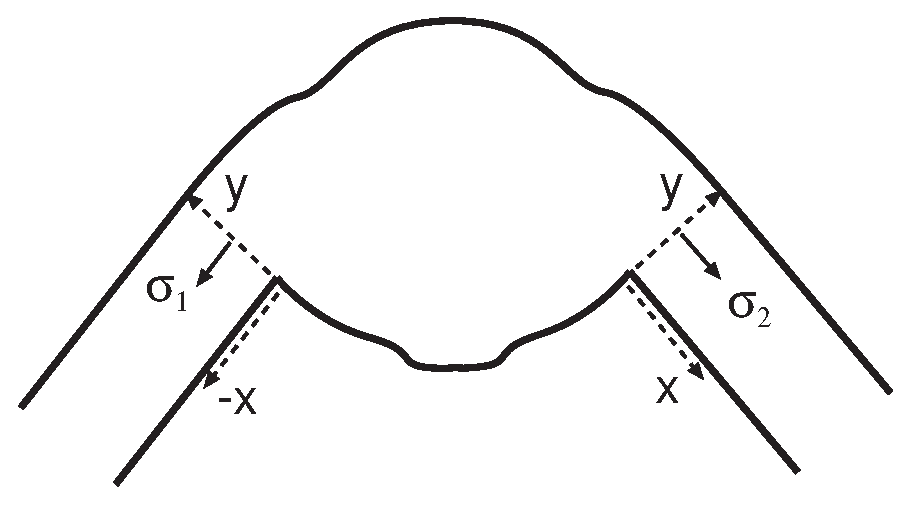
\includegraphics[width= 3in]{sprung.eps}
 \vspace{0.1 in}
 \caption{Interior region and leads.}
\end{center}
\end{figure}

%
% My working TeX directory also contained the eps file sprung.ps
%

Both of these figures ``floated'' to the top of the current page.

So it is possible to put graphics into a \LaTeX\ document, but
you may have to consult
the local expert to be sure how it's done!

\end{document}


\bye
